\section*{Question 4:}
Exercise 10.8:

Implement the nearest neighbor-based collaborative filtering algorithm. Using a publicly available collaborative filtering data set, compare the effectiveness, in terms of mean squared error, of the Euclidean distance and correlation similarity.

\subsection*{Answer:}

I downloaded the latest MovieLens small data set, ml-latest-small, from this link:

http://files.grouplens.org/datasets/movielens/ml-latest-small.zip

This data set (ml-latest-small) describes 5-star rating and free-text tagging activity from MovieLens, a movie recommendation service. It contains 100004 ratings and 1296 tag applications across 9125 movies.

These data were created by 671 users between January 09, 1995 and October 16, 2016. This dataset was generated on October 17, 2016.

Users were selected at random for inclusion. All selected users had rated at least 20 movies. No demographic information is included. Each user is represented by an id, and no other information is provided.

The data are contained in the files links.csv, movies.csv, ratings.csv and tags.csv under Q4 directory. 

I implemented the nearest neighbor-based collaborative filtering algorithm in python and saved it in the file nn.py. It takes one command line argument, which is the ratings file in csv format. The program computes MSE of Euclidean distance and correlation similarity.

\lstinputlisting[language=python, label=nn.py, caption=The content of nn.py, breakatwhitespace=〈false)]{Q4/nn.py}


\textbf{Results:}

\begin{figure}[h]
\caption{Running nn.py}
\centering
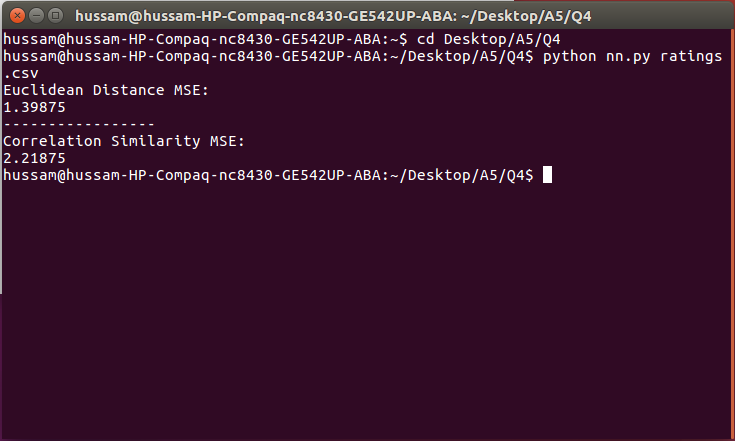
\includegraphics[scale=0.9]{Q4/nn.png}
\end{figure}

Euclidean Distance MSE = 1.39875

Correlation Similarity MSE = 2.21875

\textbf{Observation:}

The MSE of Euclidean Distance is smaller than the MSE of the Correlation Similarity. Therefore the Euclidean Distance is more effective than Correlation Similarity.
